\question{}
\begin{ابجد}
\item مسئله را به این صورت مدل‌سازی می‌کنیم:
\begin{itemize}
    \item \textbf{حالت‌ها}: هر جایگشت دلخواه از $n$ عدد مورد نظر یکی از حالت‌های مسئله هست و در کل $n!$ حالت داریم.
    \item \textbf{کنش‌ها}: طبق صورت سوال، جابه‌جایی هر دو عضو همسایه، یک کنش است. در قسمت‌های بعد، هر کنش را با $swap(i)$ نشان می‌دهیم که به معنای جابجایی اعضای $i$ ام و $i+1$ ام است.
    \item \textbf{حالت اولیه}: همان ترتیبی از اعداد که در ابتدا به ما داده شده حالت اولیۀ مسئله را تشکیل می‌دهد؛ هر یک از $n!$ جایشگت ممکن می‌تواند حالت اولیه ما باشد.
    \item \textbf{حالت نهایی}: جایگشتی که $n$ عدد مورد نظر به طور صعودی مرتب شده باشند.
\end{itemize}

\item
\begin{itemize}
    \item تابع اول: برای جایشگت $\pi$، تابع \lr{fitness} زیر را تعریف می‌کنیم:
          \begin{align*}
              f_1(\pi) = \left| \{ i \mid \pi_i = i \} \right|
          \end{align*}
          به بیان ساده‌تر، تابع $f_1$ تعداد اعدادی که در جایشگت فعلی در مکان حقیقی خود قرار دارند را نشان می‌دهد؛ بدیهی است که به ازای حالت کامل $\pi^*$، داریم $f_1(\pi^*)=n$ و به ازای هر جایگشت دیگر، $f_1<1$.
          \begin{proof}
              می‌خواهیم نشان دهیم که به ازای هر مسئله با $n \geq 3$ تابع $f_1$ حداقل یک نقطه بهینه محلی غیرسراسری دارد. جایشگت زیر را در نظر بگیرید:
              \begin{align*}
                  \pi' = (3, 2, 1, 4, 5, \dots, n)
              \end{align*}
              روشن است که:
              \begin{align*}
                  f_1(\pi') = 1 + (n-3) = n-2 \Rightarrow f_ 1(\pi') < n
              \end{align*}
              پس $\pi'$ نقطه بهینه سراسری نیست. \lr{(I)} \\
              اکشن‌های ممکن از این حالت را می‌توان به 4 دسته تقسیم کرد؛ مقدار جدید $f_1$ به ازای آنها را حساب می‌کنیم:
              \[
                  \renewcommand{\arraystretch}{1.5} % Adds vertical breathing room
                  \begin{array}{c c l l}
                      \pi' & \xrightarrow{swap(1)}         & \pi'_{new} = (2, 3, 1, 4, 5, \dots, n) & \Rightarrow f_1(\pi'_{new}) = n - 3 \\
                      \pi' & \xrightarrow{swap(2)}         & \pi'_{new} = (3, 1, 2, 4, 5, \dots, n) & \Rightarrow f_1(\pi'_{new}) = n - 3 \\
                      \pi' & \xrightarrow{swap(3)}         & \pi'_{new} = (3, 2, 4, 1, 5, \dots, n) & \Rightarrow f_1(\pi'_{new}) = n - 3 \\
                      \pi' & \xrightarrow{swap(i)_{i > 3}} & \pi'_{new} = (3, 2, 1, \dots)          & \Rightarrow f_1(\pi'_{new}) = n - 4
                  \end{array}
              \]
              همان طور که مشاهده کردیم، تمام همسایه‌های $\pi'$ مقدار \lr{fitness} کمتری نسبت به آن دارند. \lr{(II)} \\
              از \lr{(I)} و \lr{(II)} نتیجه می‌گیریم که جایشگت $\pi'$ یک نقطه بهینه محلی غیرسراسری برای $f_1$ است. از آنجا که $\pi'$ را برای هر مسئله $n \geq 3$ دلخواه در نظر گرفتیم، پس تابع $f_1$ همواره حداقل یک نقطه بهینه محلی غیرسراسری دارد.
          \end{proof}

    \item اگر $inv(\pi)$ تعداد نابجایی‌های\footnote{هر زوج $i > j$ که $\pi_i < \pi_j$ باشد را یک نابجایی یا \lr{inversion} می‌نامیم} جایگشت $\pi$ باشد، تابع \lr{fitness} جدید را به این شکل تعریف می‌کنیم:
          \begin{align*}
              f_2(\pi) = -inv(\pi)
          \end{align*}
          روشن است که برای حالت کامل $\pi^*$ داریم $f_2(\pi) = 0$ و به ازای هر جایگشت دیگر $f_2 < 0$.
          \begin{proof}
              نشان می‌دهیم که به ازای هیچ $n \geq 3$، تابع $f_2$ نقطه بهینه محلی غیرسراسری ندارد. \\
              فرض کنید $\pi \neq \pi^*$ یک جایشگت مسئله باشد. ادعا می‌کنیم $1 \leq i < n$ وجود دارد به طوری که $\pi_{i+1} < \pi_i$؛ اگر چنین نباشد، آنگاه می‌توان نتیجه گرفت که $\pi_1 < \pi_2 < \dots < \pi_n$ که در این صورت شرط $\pi \neq \pi^*$ نقض می‌شود. \\
              پس $(i, i+1)$ یک نابجایی در جایگشت $\pi$ است. حال اگر اکشن $swap(i)$ را انجام دهیم، این نابجایی حذف می‌شود. از طرف دیگر با این اکشن، هیچ تغییری در نابجایی‌های به شکل ${(i, j)}_{j \neq i + 1}$ و ${(j, i + 1)}_{j \neq i}$ به وجود نمی‌آید. پس داریم:
              \begin{align*}
                  f_2(\pi_{new}) = f_2(\pi) + 1
              \end{align*}
              پس هیچ جایشگت $\pi \neq \pi^*$ نمی‌تواند یک نقطه بهینه محلی باشد. پس به ازای این تابع \lr{fitness}، نقطه بهینه محلی غیرسراسری نداریم.
          \end{proof}
\end{itemize}

\item در هر مرحله، به ترتیب اکشن‌های $swap(1)$، $swap(2)$ و $swap(3)$ را انجام می‌دهیم تا همسایه‌های حالت فعلی را بسازیم؛ سپس یکی از همسایه‌ها با بالاترین میزان \lr{fitness} را انتخاب می‌کنیم. اگر هیچ همسایه‌ای \lr{fitness} بهتر از حالت فعلی نداشت، الگوریتم خاتمه می‌یابد. اگر هم چند همسایه بالاترین میزان \lr{fitness} را داشتند، اولویت با همسایه‌ای هست که زودتر ساخته شده.
\begin{figure}[H]
    \centering
    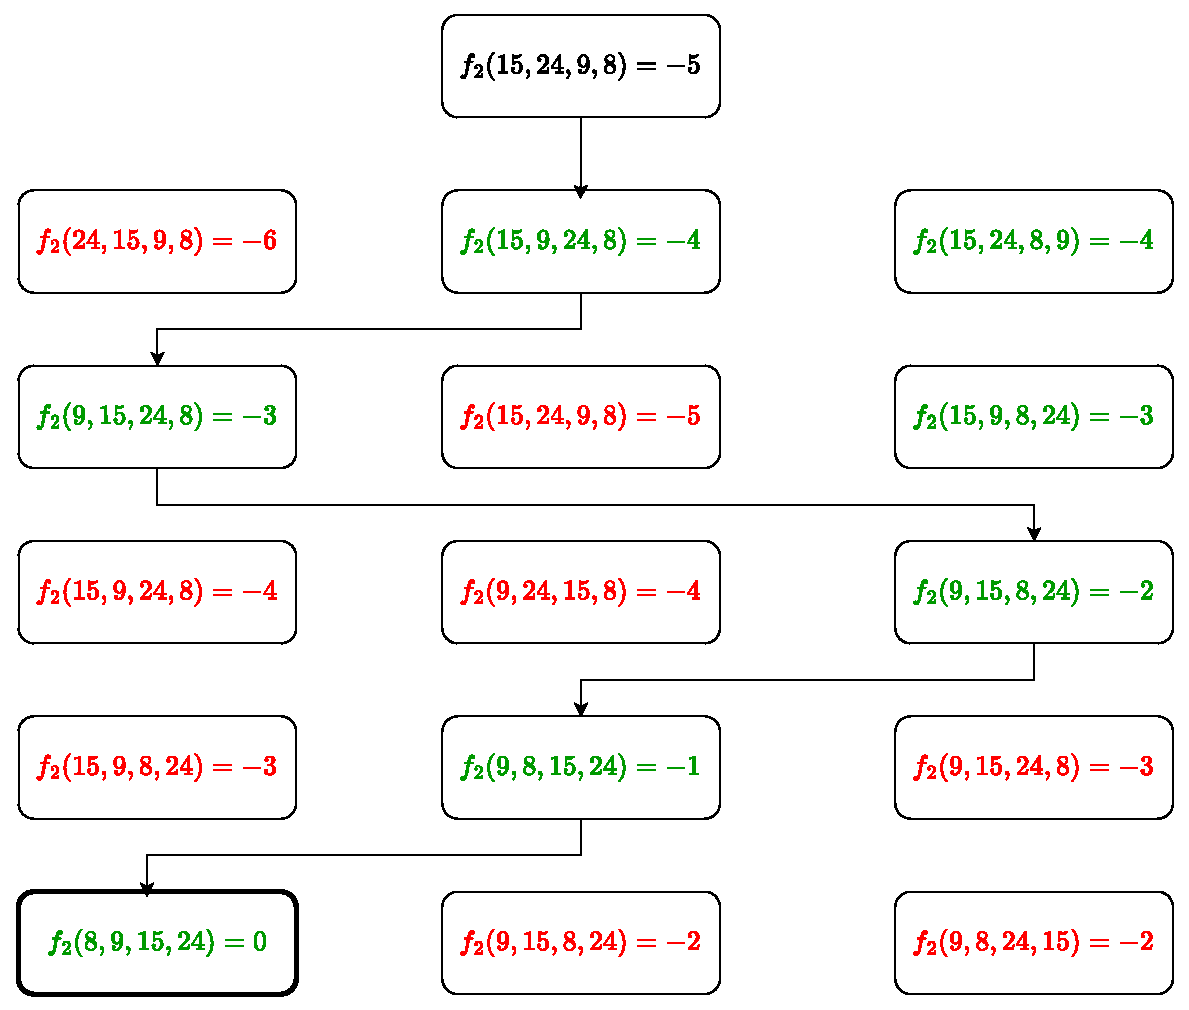
\includegraphics[width=0.7\textwidth]{assets/hill_climbing.pdf}
    \vspace{0.4cm}
    \label{fig:hill climbing}
\end{figure}
به علت ویژگی \lr{involution} اکشن‌ها در این مسئله که اگر یک اکشن را دو بار به صورت متوالی روی یک حالت انجام دهیم دوباره به حالت اولیه برمی‌گردیم، همواره یکی از همسایه‌های تولید شده \lr{fitness} بدتری نسبت به حالت فعلی دارد و می‌توانستیم اصلا آن را تولید نکنیم. \\
همچنین همان طور که در قسمت قبل اشاره شد، هر اکشن میزان \lr{fitness} را تنها یک واحد تغییر می‌دهد، و از طرفی نقطه بهینه محلی غیرسراسری هم نداریم. پس می‌توانیم در هر مرحله یک نابجایی بین دو عضو متوالی را پیدا کرده و آنها را \lr{swap} کنیم. در این صورت دیگر نیازی به تولید همه همسایه‌ها نبود.

\pagebreak

\item الگوریتم \lr{Simulated Annealing} را اجرا می‌کنیم:
\begin{itemize}
    \item \textbf{مرحله 1 ($t=1$)}:
          \begin{itemize}
              \item \textbf{حالت فعلی:} $\pi = (15, 24, 9, 8)$ | $T = 5$ | $f_2(\pi) = -5$
              \item \textbf{همسایه ($swap(1)$):} $\pi' = (24, 15, 9, 8)$ | $f_2(\pi') = -6$
                    \begin{itemize}
                        \item $\Delta E = f_2(\pi') - f_2(\pi) = (-6) - (-5) = -1$
                        \item محاسبه احتمال پذیرش: $P = e^{\Delta E / T} = e^{-1/5} \approx 0.818$
                        \item عدد تصادفی مصرف شده: $r = 0.27$
                        \item \textbf{نتیجه:} چون $r \le P$، این همسایه پذیرفته می‌شود.
                    \end{itemize}
          \end{itemize}

          \vspace{0.7cm}

    \item \textbf{مرحله 2 ($t=2$)}:
          \begin{itemize}
              \item \textbf{حالت فعلی:} $\pi = (24, 15, 9, 8)$ | $T = 4$ | $f_2(\pi) = -6$
              \item \textbf{همسایه ($swap(1)$):} $\pi' = (15, 24, 9, 8)$ | $f_2(\pi') = -5$
                    \begin{itemize}
                        \item $\Delta E = f_2(\pi') - f_2(\pi) = (-5) - (-5) = 1$
                        \item \textbf{نتیجه:} این همسایه بهتر از حالت فعلی بوده و انتخاب می‌شود.
                    \end{itemize}
          \end{itemize}

          \vspace{0.7cm}

    \item \textbf{مرحله 3 ($t=3$)}:
          \begin{itemize}
              \item \textbf{حالت فعلی:} $\pi = (15, 24, 9, 8)$ | $T = 3$ | $f_2(\pi) = -5$
              \item \textbf{همسایه ($swap(1)$):} $\pi' = (24, 15, 9, 8)$ | $f_2(\pi') = -6$
                    \begin{itemize}
                        \item $\Delta E = f_2(\pi') - f_2(\pi) = (-6) - (-5) = -1$
                        \item محاسبه احتمال پذیرش: $P = e^{\Delta E / T} = e^{-1/3} \approx 0.716$
                        \item عدد تصادفی مصرف شده: $r = 0.66$
                        \item \textbf{نتیجه:} چون $r \le P$، این همسایه پذیرفته می‌شود.
                    \end{itemize}
          \end{itemize}

          \vspace{0.7cm}

    \item \textbf{مرحله 4 ($t=4$)}:
          \begin{itemize}
              \item \textbf{حالت فعلی:} $\pi = (24, 15 9, 8)$ | $T = 2$ | $f_2(\pi) = -6$
              \item \textbf{همسایه ($swap(1)$):} $\pi' = (15, 24, 9, 8)$ | $f_2(\pi') = -5$
                    \begin{itemize}
                        \item $\Delta E = f_2(\pi') - f_2(\pi) = (-5) - (-6) = 1$
                        \item \textbf{نتیجه:} این همسایه بهتر از حالت فعلی بوده و انتخاب می‌شود.
                    \end{itemize}
          \end{itemize}

          \vspace{0.7cm}

    \item \textbf{مرحله 5 ($t=5$)}:
          \begin{itemize}
              \item \textbf{حالت فعلی:} $\pi = (15, 24, 9, 8)$ | $T = 1$ | $f_2(\pi) = -5$
              \item \textbf{همسایه ($swap(1)$):} $\pi' = (24, 15, 9, 8)$ | $f_2(\pi') = -6$
                    \begin{itemize}
                        \item $\Delta E = f_2(\pi') - f_2(\pi) = (-6) - (-5) = -1$
                        \item محاسبه احتمال پذیرش: $P = e^{\Delta E / T} = e^{-1/1} \approx 0.367$
                        \item عدد تصادفی مصرف شده: $r = 0.91$
                        \item \textbf{نتیجه:} چون $r > P$، این همسایه پذیرفته نمی‌شود و در مرحله بعد، همسایه بعدی را بررسی می‌کنیم.
                    \end{itemize}
          \end{itemize}

          \vspace{0.7cm}

    \item \textbf{مرحله 6 ($t=6$)}:
          \begin{itemize}
              \item \textbf{حالت فعلی:} $\pi = (15, 24, 9, 8)$ | $T = 0$ | $f_2(\pi) = -5$
              \item \textbf{همسایه ($swap(2)$):} $\pi' = (15, 9, 24, 8)$ | $f_2(\pi') = -4$
                    \begin{itemize}
                        \item $\Delta E = f_2(\pi') - f_2(\pi) = (-4) - (-5) = 1$
                        \item \textbf{نتیجه:} این همسایه بهتر است و انتخاب می‌شود.
                    \end{itemize}
          \end{itemize}

          \vspace{0.7cm}

    \item \textbf{مرحله 7 ($t=7$)}:
          \begin{itemize}
              \item \textbf{حالت فعلی:} $\pi = (15, 9, 24, 8)$ | $T = 0$ | $f_2(\pi) = -4$
              \item \textbf{همسایه ($swap(1)$):} $\pi' = (9, 15, 24, 8)$ | $f_2(\pi') = -3$
                    \begin{itemize}
                        \item $\Delta E = f_2(\pi') - f_2(\pi) = (-3) - (-4) = 1$
                        \item \textbf{نتیجه:} این همسایه بهتر است و انتخاب می‌شود.
                    \end{itemize}
          \end{itemize}

          \vspace{0.7cm}

    \item \textbf{مرحله 8 ($t=8$)}:
          \begin{itemize}
              \item \textbf{حالت فعلی:} $\pi = (9, 15, 24, 8)$ | $T = 0$ | $f_2(\pi) = -3$
              \item \textbf{همسایه ($swap(1)$):} $\pi' = (15, 9, 24, 8)$ | $f_2(\pi') = -4$
                    \begin{itemize}
                        \item $\Delta E = f_2(\pi') - f_2(\pi) = (-4) - (-3) = -1$
                        \item \textbf{نتیجه:} در این مرحله $T=0$ بنابراین همسایه بدتر انتخاب نمی‌شود.
                    \end{itemize}
          \end{itemize}

          \vspace{0.7cm}
\end{itemize}

الگوریتم بدون رسیدن به حالت هدف، خاتمه یافت.

\end{ابجد}